\documentclass{article}

\usepackage{booktabs} 
\usepackage[english]{babel}
\usepackage{graphicx}
\usepackage{amsmath}
\usepackage{listings}
\usepackage{url}

\title {Project Report}
\date{21 December 2016}
\author{Elise Mol, Wendy Nieuwkamer, and Isobel Smith}

\begin{document}

\maketitle

\section{Problem}
	
	After three months of learning about several machine learning techniques and classifying algorithms it was time to put our newly gained skills into practice. We decided to try our hand at one of the competitions hosted by Kaggle. The challenge we chose is Leaf Classification; the objective of the competition is to use binary leaf images and their extracted features to predict what species each leaf belongs to. The dataset which was provided includes around 1584 images of leaf specimens; these samples include 99 species. From every image three sets of features are extracted: a shape contiguous descriptor, an interior texture histogram and a fine-scale margin histogram. Every feature is represented as a 64-attribute vector. 
	
	As the competition started at 30 August 2016, there were already quite some submissions made and kernels active. One of them stood out, namely "10 Classifier Showdown in Scikit-Learn". In this kernel Jeff Delaney compared ten classifiers which are part of the python library Scikit-Learn. The results of his experiment are shown in figure \ref{fig:showdown}. In his experiment Delaney used the default setup for the classifiers , combined with semi-random parameters. He notes that the performance of the classifiers could be improved by tuning the hyper-parameters. Thus, our research question is whether we can improve the accuracy found by Delaney by tuning the hyper-parameters of the classifiers.
	
	\begin{figure} 
		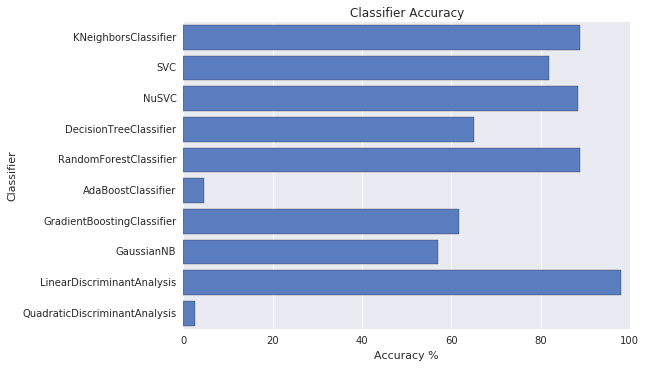
\includegraphics[width=\linewidth]{results-showdown.png}
		\caption{The 10 Classifier Showdown}
		\label{fig:showdown}
	\end{figure}
	
	As we did not have time to run experiments for all ten classifiers, we decided to look into five of them. We chose the K-neigbors classifier, decision tree classifier and Gaussian Naive Bayes as they had relatively decent accuracy at respectively 88\%, 65\%, and 57\%. Also, we had some background in these algorithms as they had been taught in our Machine Learning course. Additionally, we decided to choose either Ada boost or quadratic discriminant analysis as they could improve the most with found accuracies of 4.5\% and 2.5\%. 

\newpage
\section{The algorithms}
	Before we could start optimizing the hyper-parameters we had to research the algorithms we chose. In order to discover the most relevant information for our experiment we aimed to answer the following questions:
	
	\begin{itemize}
		\item How does the classifier work? 
		\item Which hyper-parameters exist for each classifier?
		\item Which hyper-parameters have the most effect on the classifier?
	\end{itemize}
	
	The answers to these questions are specific to the Scikit-Learn package.
	
	\subsection{K-neighbors}
		The k-neighbors algorithm classifies an object according to the k nearest objects from the training set. For a higher k noise might be filtered out, but class boundaries might become more vague and less accurate. Thus, it would be interesting to find out which value of k gives the highest accuracy for our dataset. There are two ways of computing the class from the neigbors. The first one is by giving all the neighbors equal weight, no matter how far or close they are.  The second is to give each neighbor a weight relative to its distance. The weighted version of the 
	
	\subsection{Decision Tree Classifier}
	
	\subsection{Gaussian Naive Bayes}
WE did not choose this because....
	
	\subsection{Ada Boost Classifier}
	
	\subsection{Quadratic Discriminant Analysis}
we did not choose this because ....


\section{Hyper parameter optimization}

	The goal of hyper parameter optimization is to find the best hyperparameters for the given classifier, in order to optimise the loss function and to avoid overfitting \cite{Bergstra}. Hyperparameter optimization is one of the most important steps in machine learning \cite{bardenet}. Some hyper parameter optimisation algorithms not only find the best hyperparameters, but identify those that carry the most weight, \cite{Bergstra}.
	We needed an algorithm to find the best way to tune the hyper parameters of our chosen classifiers.  As we were recommended grid search, this was the algorithm we decided to look into.  
	
	\subsection{Grid Search}
	
		Grid Search is an algorithm for hyperparameter optimisation. It does this by iterating over all of the variables in a given range, and selecting the best combination to use in the chosen classifier. 
		As grid search was recommended to us, and is the most widely used way to optimize hyper parameters, we decided to use it in our project.
		
	\subsection{Grid Search in Scikit-Learn}
	
		Scikit-Learn has a built in function for Grid Search \cite{gridsearch}, which is defined below:
		
		
	\begin{lstlisting}
GridSearchCV(estimator, param_grid, scoring=None, fit_params=None, 
   n_jobs=1, iid=True, refit=True, cv=None, verbose=0, 
   pre_dispatch='2*n_jobs', error_score='raise',
   return_train_score=True)
	\end{lstlisting}
		
		The param \textunderscore grid is a dictionary of the parameters you want to choose and the range of parameters to try. The grid search algorithm will then run the given classifier over the entire parameter grid for the best possible combination. 
		
		Scoring allows you to choose to train for precision or recall. Precision is the fraction of retrieved instances that are relevant, whilst recall is the fraction of relevant instances that are retrieved.
		
		\begin{align*}
		Precision &= true positive / true positive + false positive\\
		Recall &= true positive / true positive + false negative 
		\end{align*}
		
		We decided to focus on precision, as we wanted to tune accurate classifiers. 
		
		The output of GridSearch is the a dict, with the names of the hyperparamter as keys, and the optimal result as values. 
		
		\begin{lstlisting}
{hyperparameter: optimal value, hyperparameter: optimal value}
		\end{lstlisting}


	\subsection{Application of GridSearch}




\newpage
\section{Results}

The accuracy of classifiers with optimized hyper-parameters were graphed against those without optimized hyper-parameters:

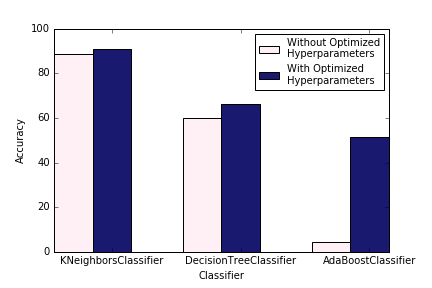
\includegraphics[scale=0.7]{acc_class}

In each of the cases, grid search clearly improved the accuracy of the classifier. This highlights the importance of hyperparameter optimisation. 
\section{Evaluation of Approach and Solution} 
	How could we have done this better/differently?
	Problems we ran into: learning curves of the algorithms.
	Possibilities for further improvement/research.
	

\bibliographystyle{unsrt}
\bibliography{ProjectReportSources}


\section{Sources}


https://www.kaggle.com/jeffd23/leaf-classification/10-classifier-showdown-in-scikit-learn



















\end{document}